\documentclass[11pt, professionalfonts]{beamer}
\usetheme[
	% sectionpage=progressbar,
	% subsectionpage=progressbar,
	progressbar=head]{metropolis}

\useoutertheme{infolines}
% \useinnertheme{rounded}
\usecolortheme{beaver}



\usepackage{longtable}
\usepackage{newtxtext,newtxmath}
\usepackage[backend=biber,style=gb7714-2015, gbnamefmt=lowercase, 
maxcitenames=2,
mincitenames=1, 
gbcitelocal=gb7714-2015,
gbpub=false,
doi=false,
isbn=false,
url=false,
eprint=false]{biblatex}
\addbibresource{yy.bib}
\hypersetup{pdfpagemode=FullScreen}
\usepackage{ctex}
\setmainfont{Times New Roman}
\setCJKmainfont[ItalicFont=华文楷体,BoldFont=华文细黑]{华文宋体}
\usepackage{graphicx}
\usepackage{amsmath}
\usepackage{amsfonts}
\usepackage{subfigure}
\usepackage{url}
\definecolor{awesome}{rgb}{1.0, 0.13, 0.32}
% \usepackage{mathptm}
\numberwithin{equation}{section}
\usefonttheme[onlymath]{serif}
% \setlength{\parskip}{1.2em}
\DeclareGraphicsExtensions{.eps,.ps,.jpg,.bmp,.png}

\author{统计71~~王泽昊}
\institute{指导教师: 张春霞}

\date{2021年4月21日}

\title{数学与统计学院~毕业设计}
\subtitle[本科毕业设计]{聚类算法在地震速度谱自动拾取中的应用研究}

\graphicspath{{images/}}


\begin{document}
{\usebackgroundtemplate{
\includegraphics[height=\paperheight,width=\paperwidth]{background.png}}
\songti
\maketitle

\begin{frame}
    \frametitle{主要工作}
    \begin{itemize}
        \item 文献调研 \& 指定外文文献翻译; 
        \item 相关背景知识学习; 
        \item 聚类算法理论学习; 
        \item 代码编写 \& 试验; 
        \item 后续改进. 
    \end{itemize}
\end{frame}

\begin{frame}[shrink]
    \frametitle{文献调研}
    \vspace{10pt}
    通过约20篇的文献调研, 了解到以往NMO速度分析有以下几种方法: 
    
    \vspace{40pt}
    \begin{center}
        \begin{minipage}{.35\textwidth}
            \begin{itemize}
                \item 速度谱相似性; 
                \item 局部地震斜率; 
                \item 神经网络; 
                \item 聚类. 
            \end{itemize}
        \end{minipage}
    \end{center}
\end{frame}

\begin{frame}[shrink]
    \frametitle{文献翻译}
    \vspace{20pt}
    对下列两篇文献进行了全文翻译. 

    \vspace{20pt}
    \citetitle{Zhang2016}\cite{Zhang2016}
    
    \vspace{20pt}
    \citetitle{Rodriguez2014}\cite{Rodriguez2014}
\end{frame}

\begin{frame}
    \frametitle{背景知识学习}
    由于地震勘探学背景知识的缺乏, 对此书籍进行了学习: 

    \vspace{20pt}
    \fullcite{Zhou2014}\cite{Zhou2014}
\end{frame}

\printbibliography

% \section{背景介绍}
\begin{frame}{地震波探测}
    \begin{figure}[ht]
        \centering
        \subfigure[共中点道集]{
            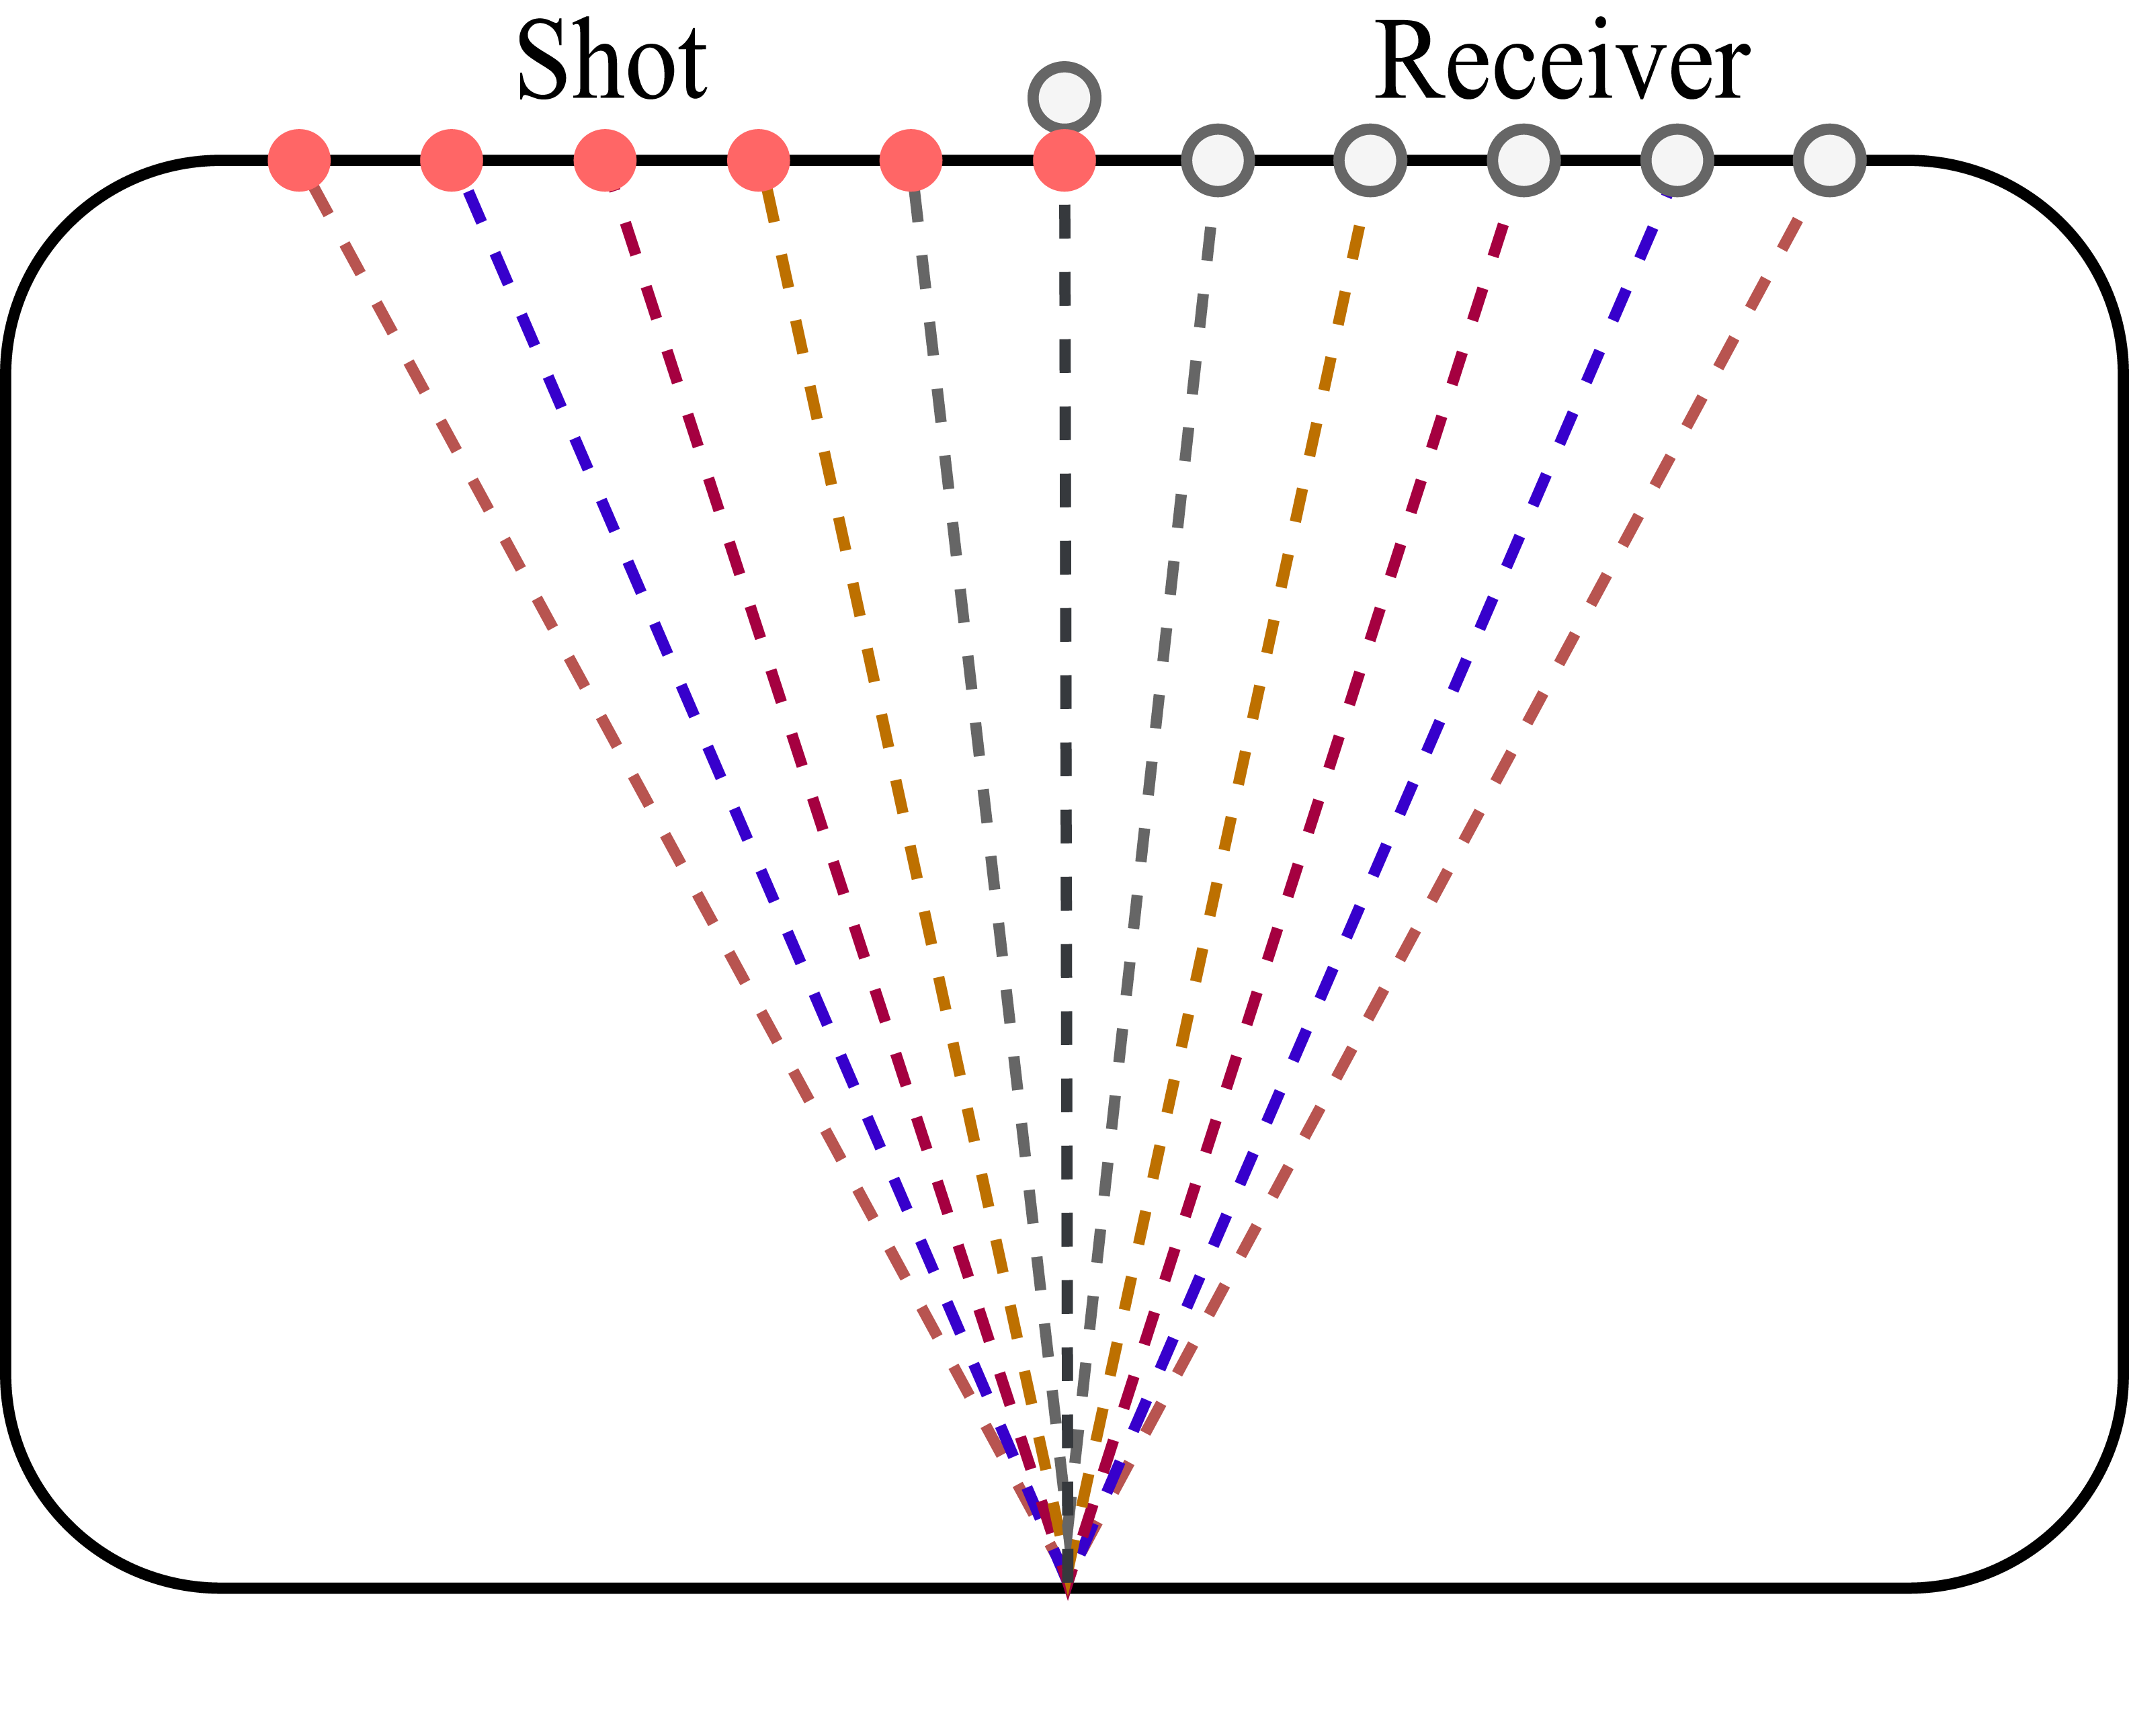
\includegraphics[height=4cm]{03_共中点道集.png}
        }\ 
        \subfigure[旅行时与偏移距的关系]{
            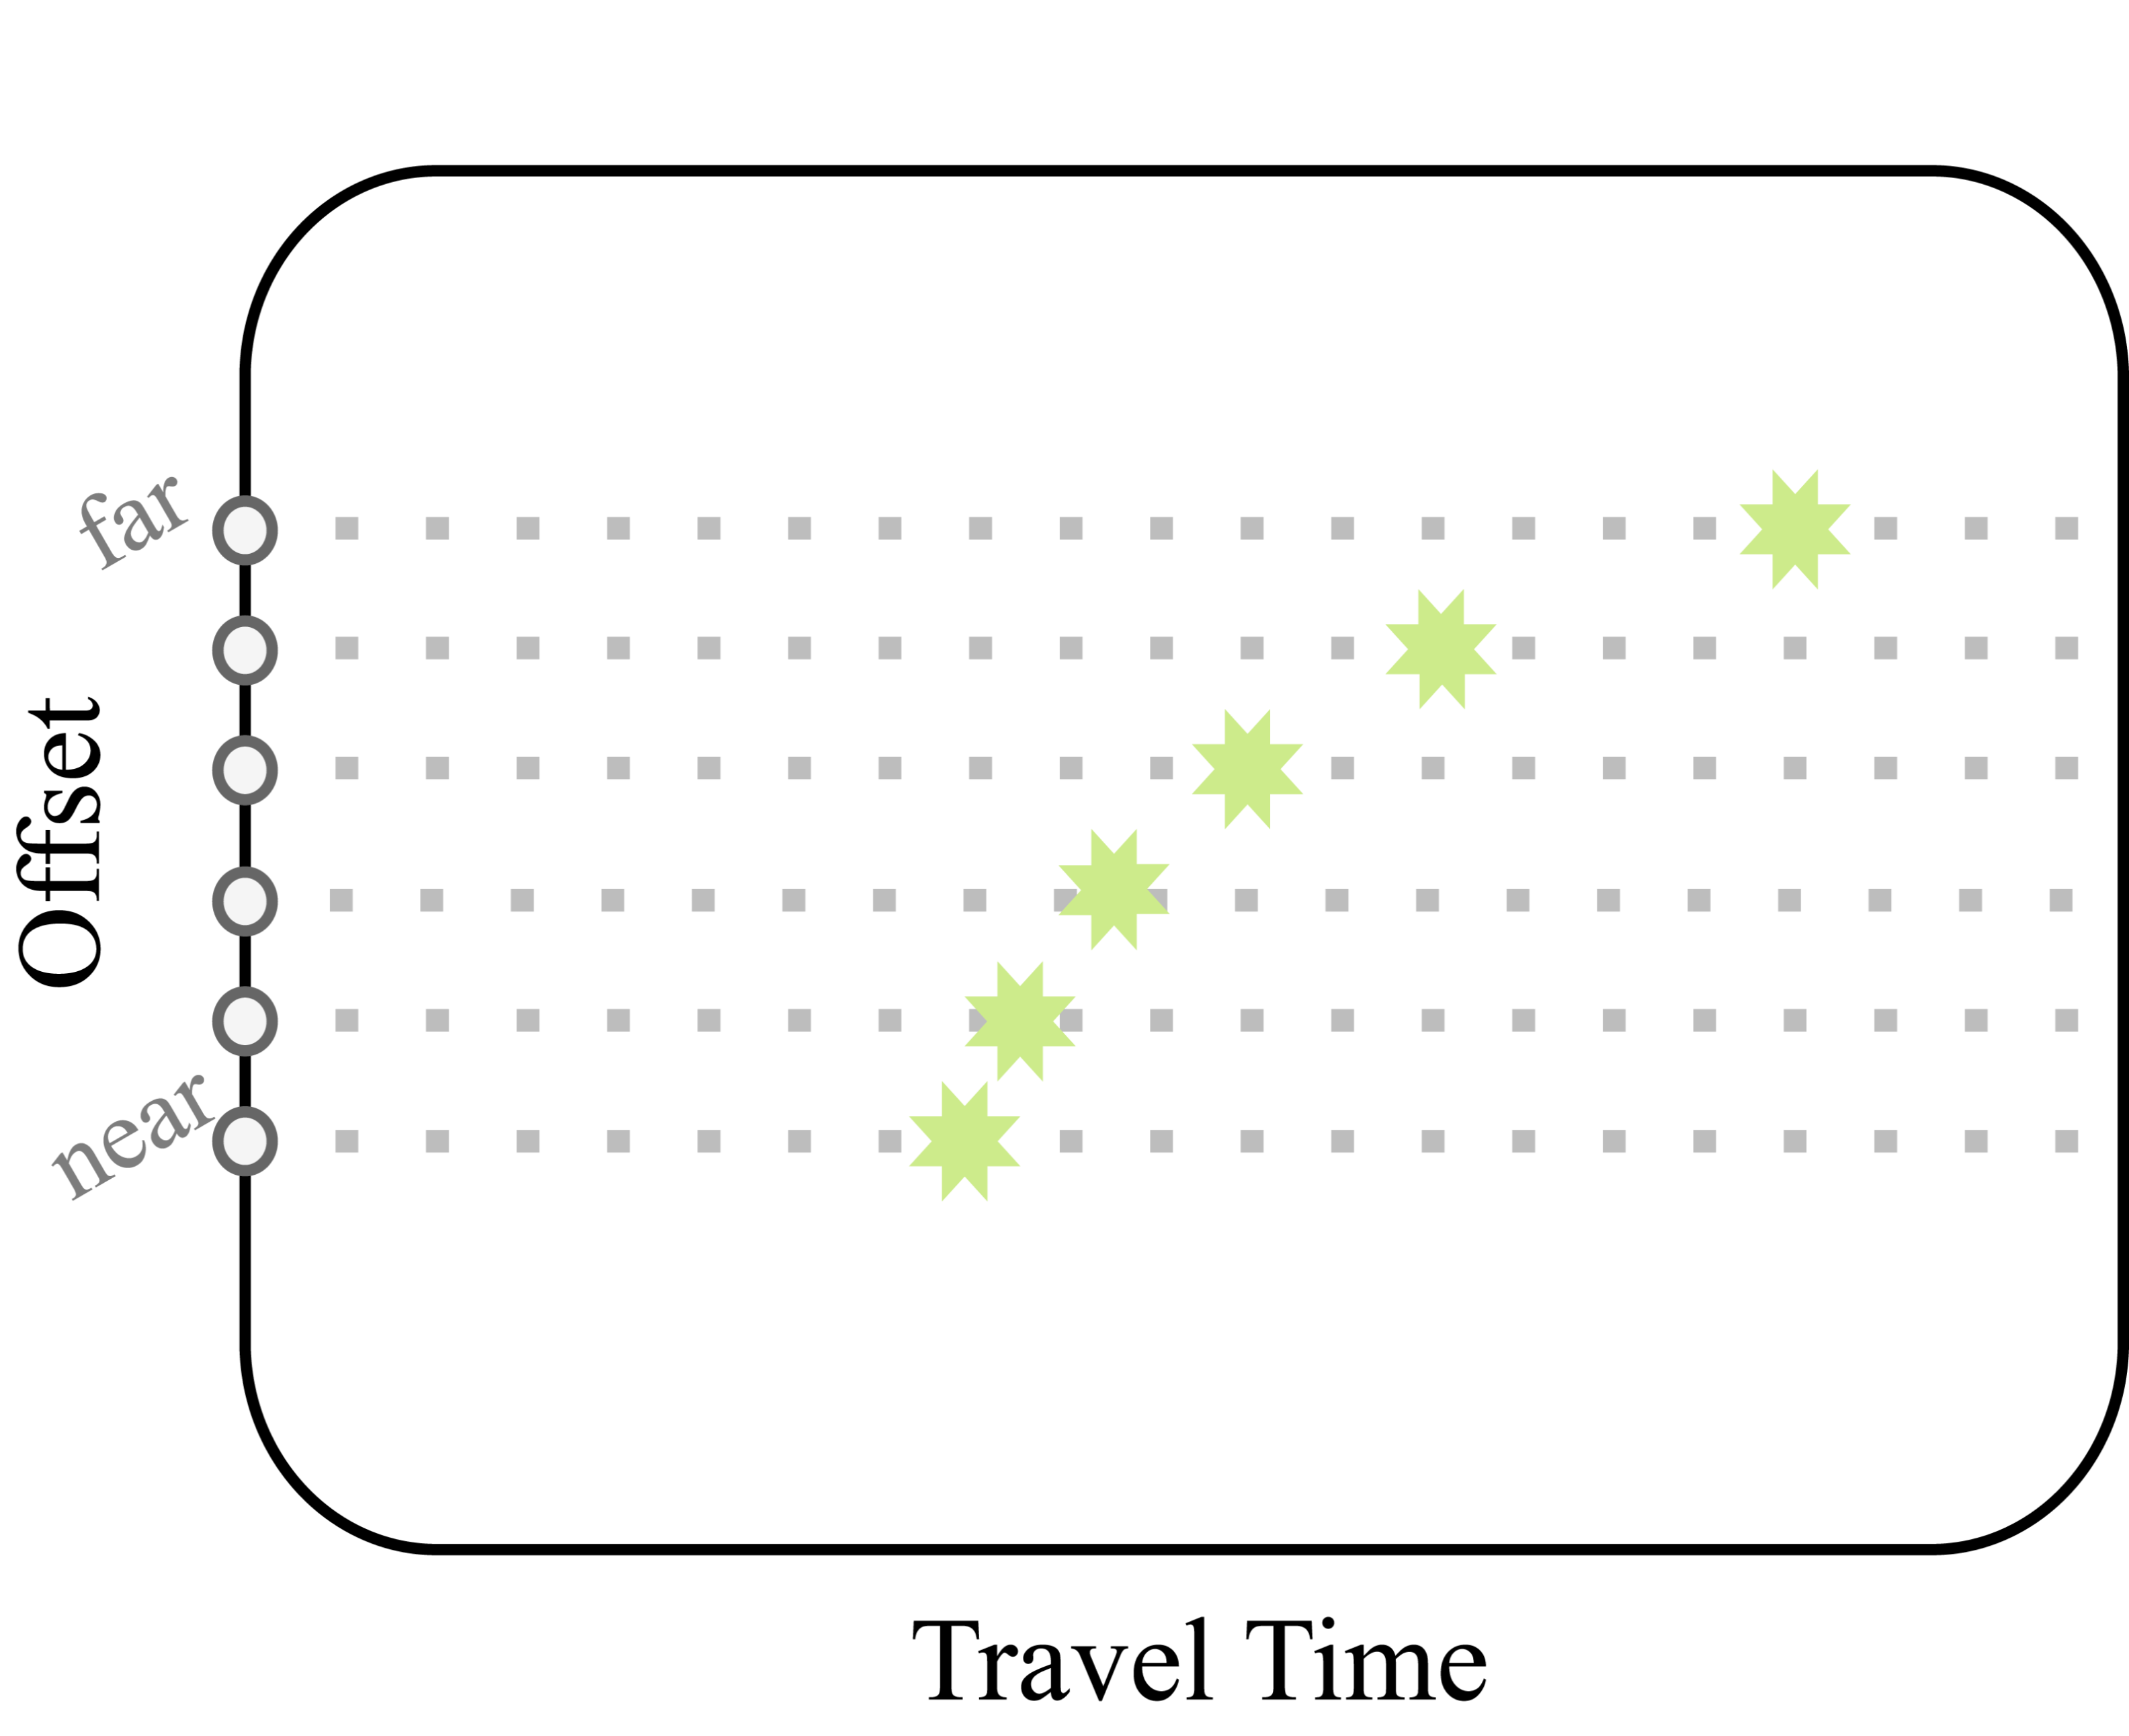
\includegraphics[height=4cm]{04_偏移距与旅行时图像_NMO前_copy.png}
        }
    \end{figure}
\end{frame} 

\begin{frame}{动校正}
    \begin{figure}[ht]
        \centering
        \subfigure[NMO前旅行时与偏移距的关系]{
            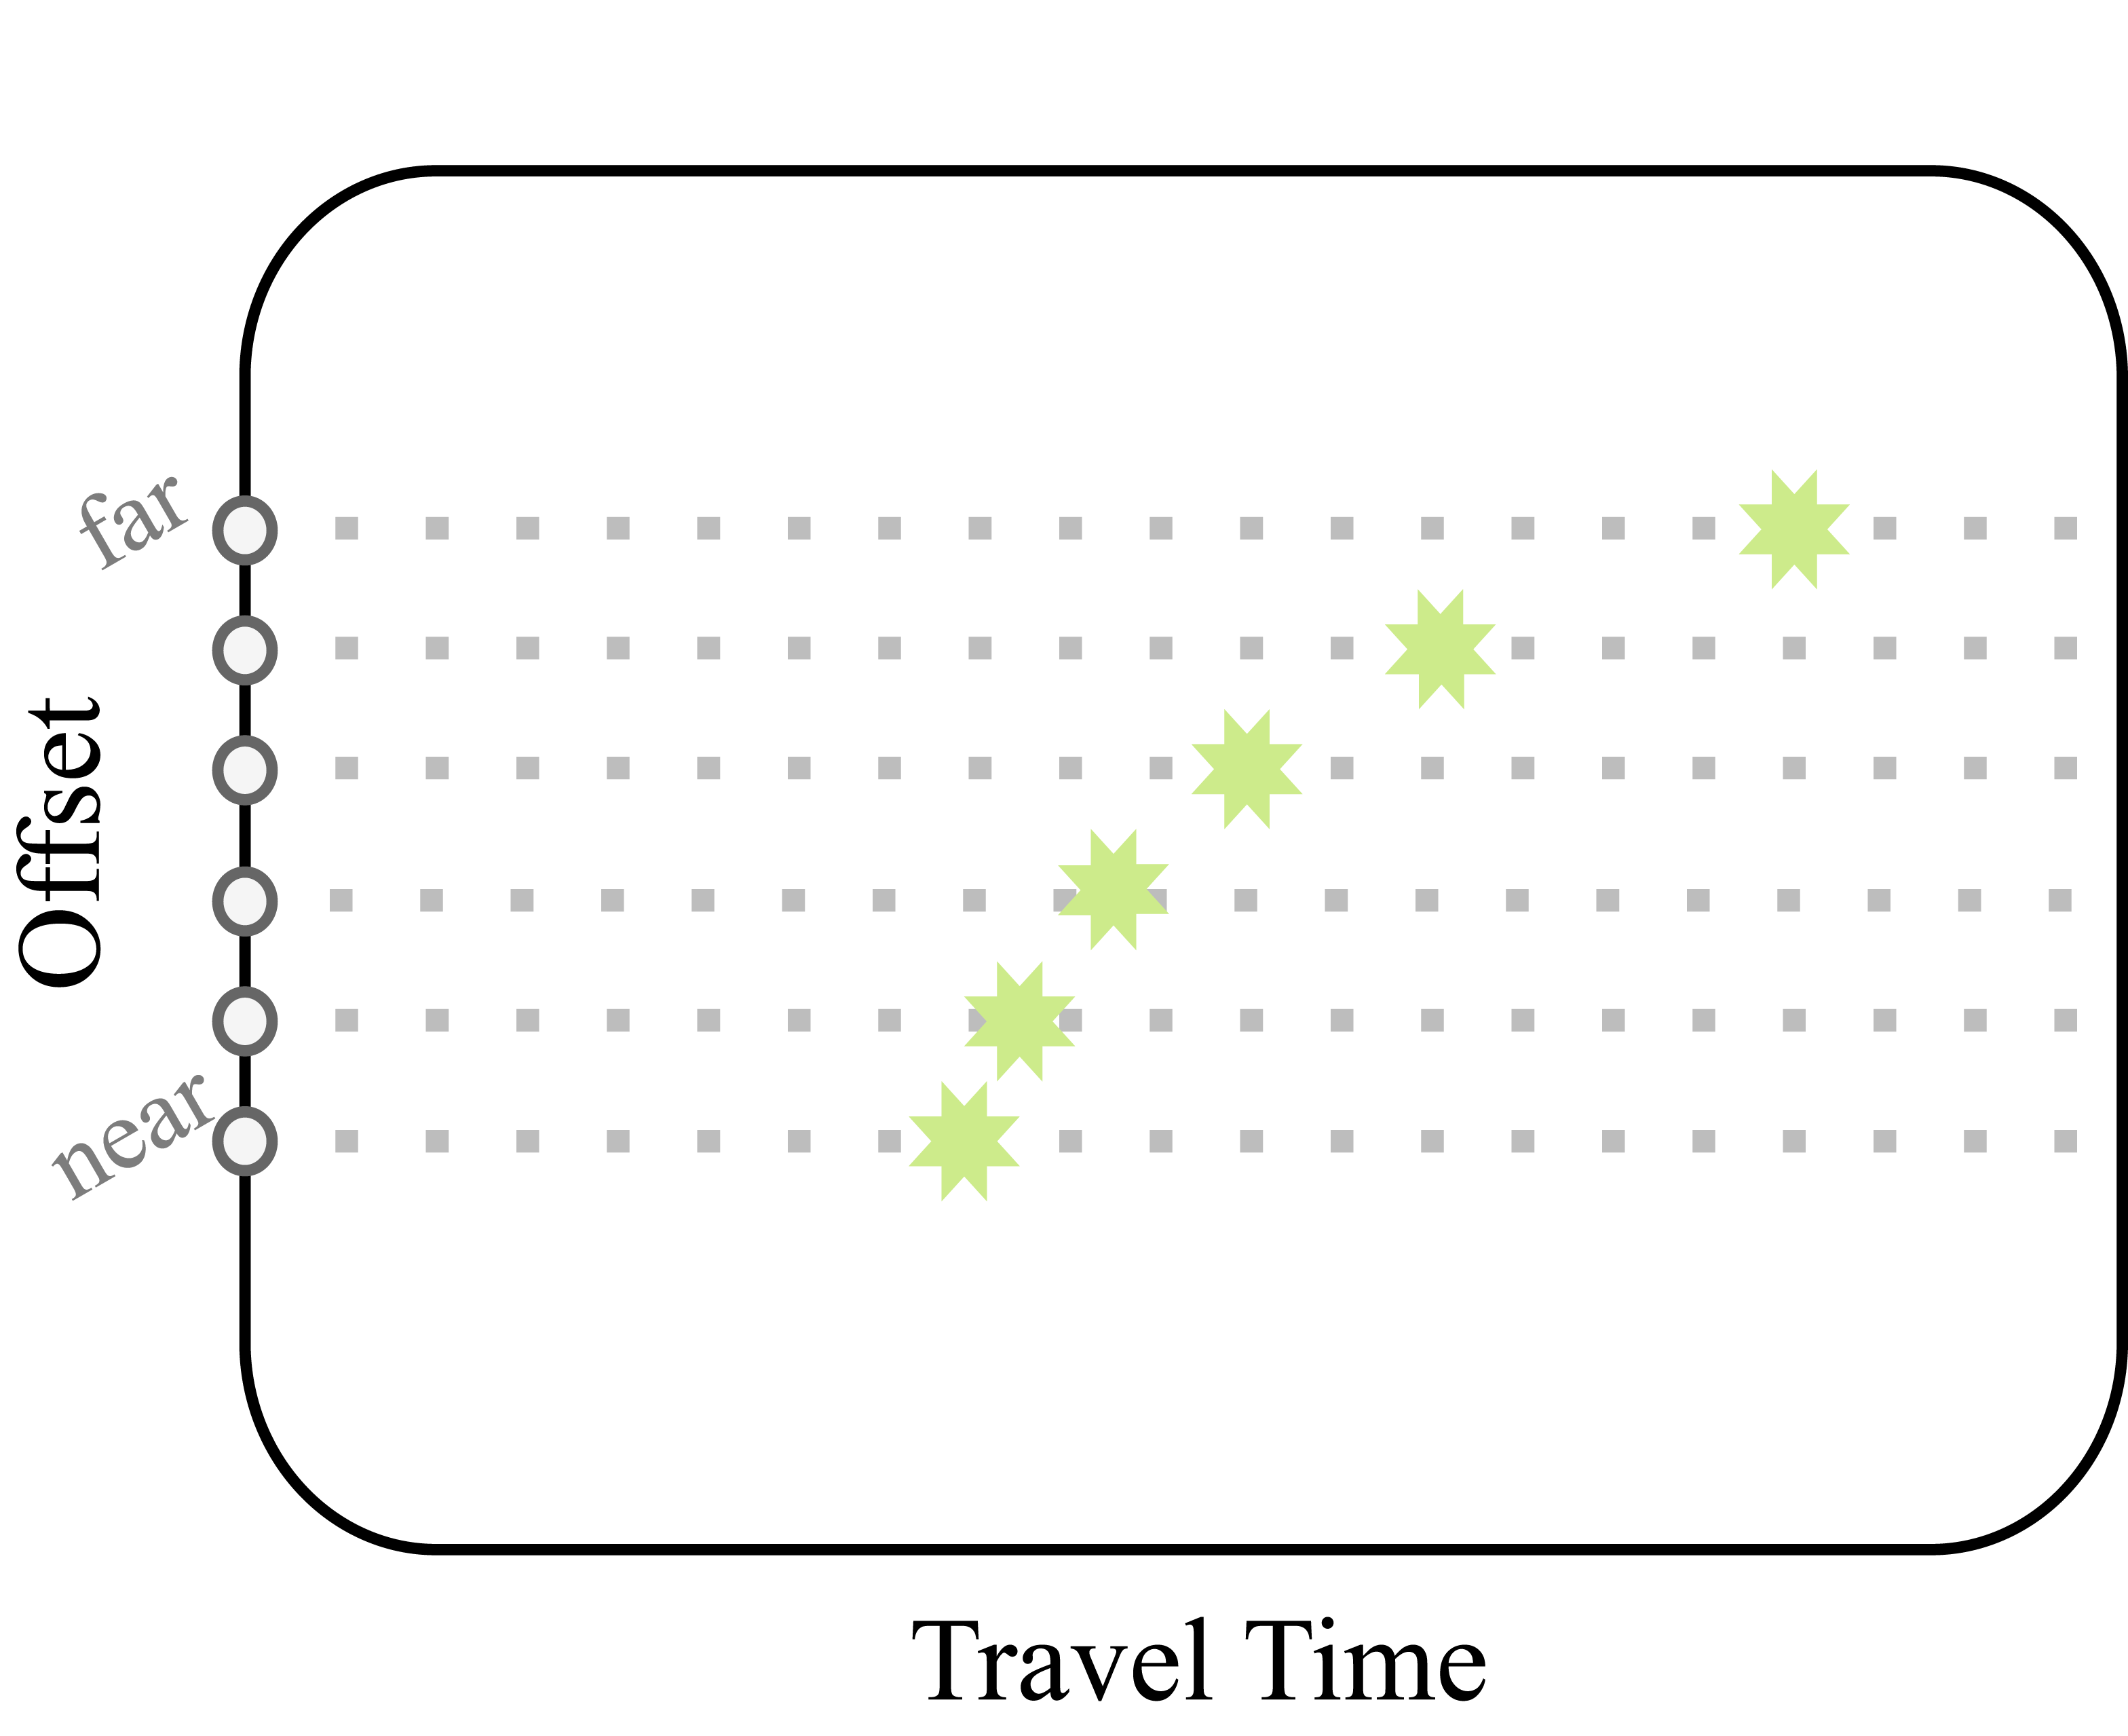
\includegraphics[height=4cm]{04_偏移距与旅行时图像_NMO前.png}
        }\ 
        \subfigure[NMO后旅行时与偏移距的关系]{
            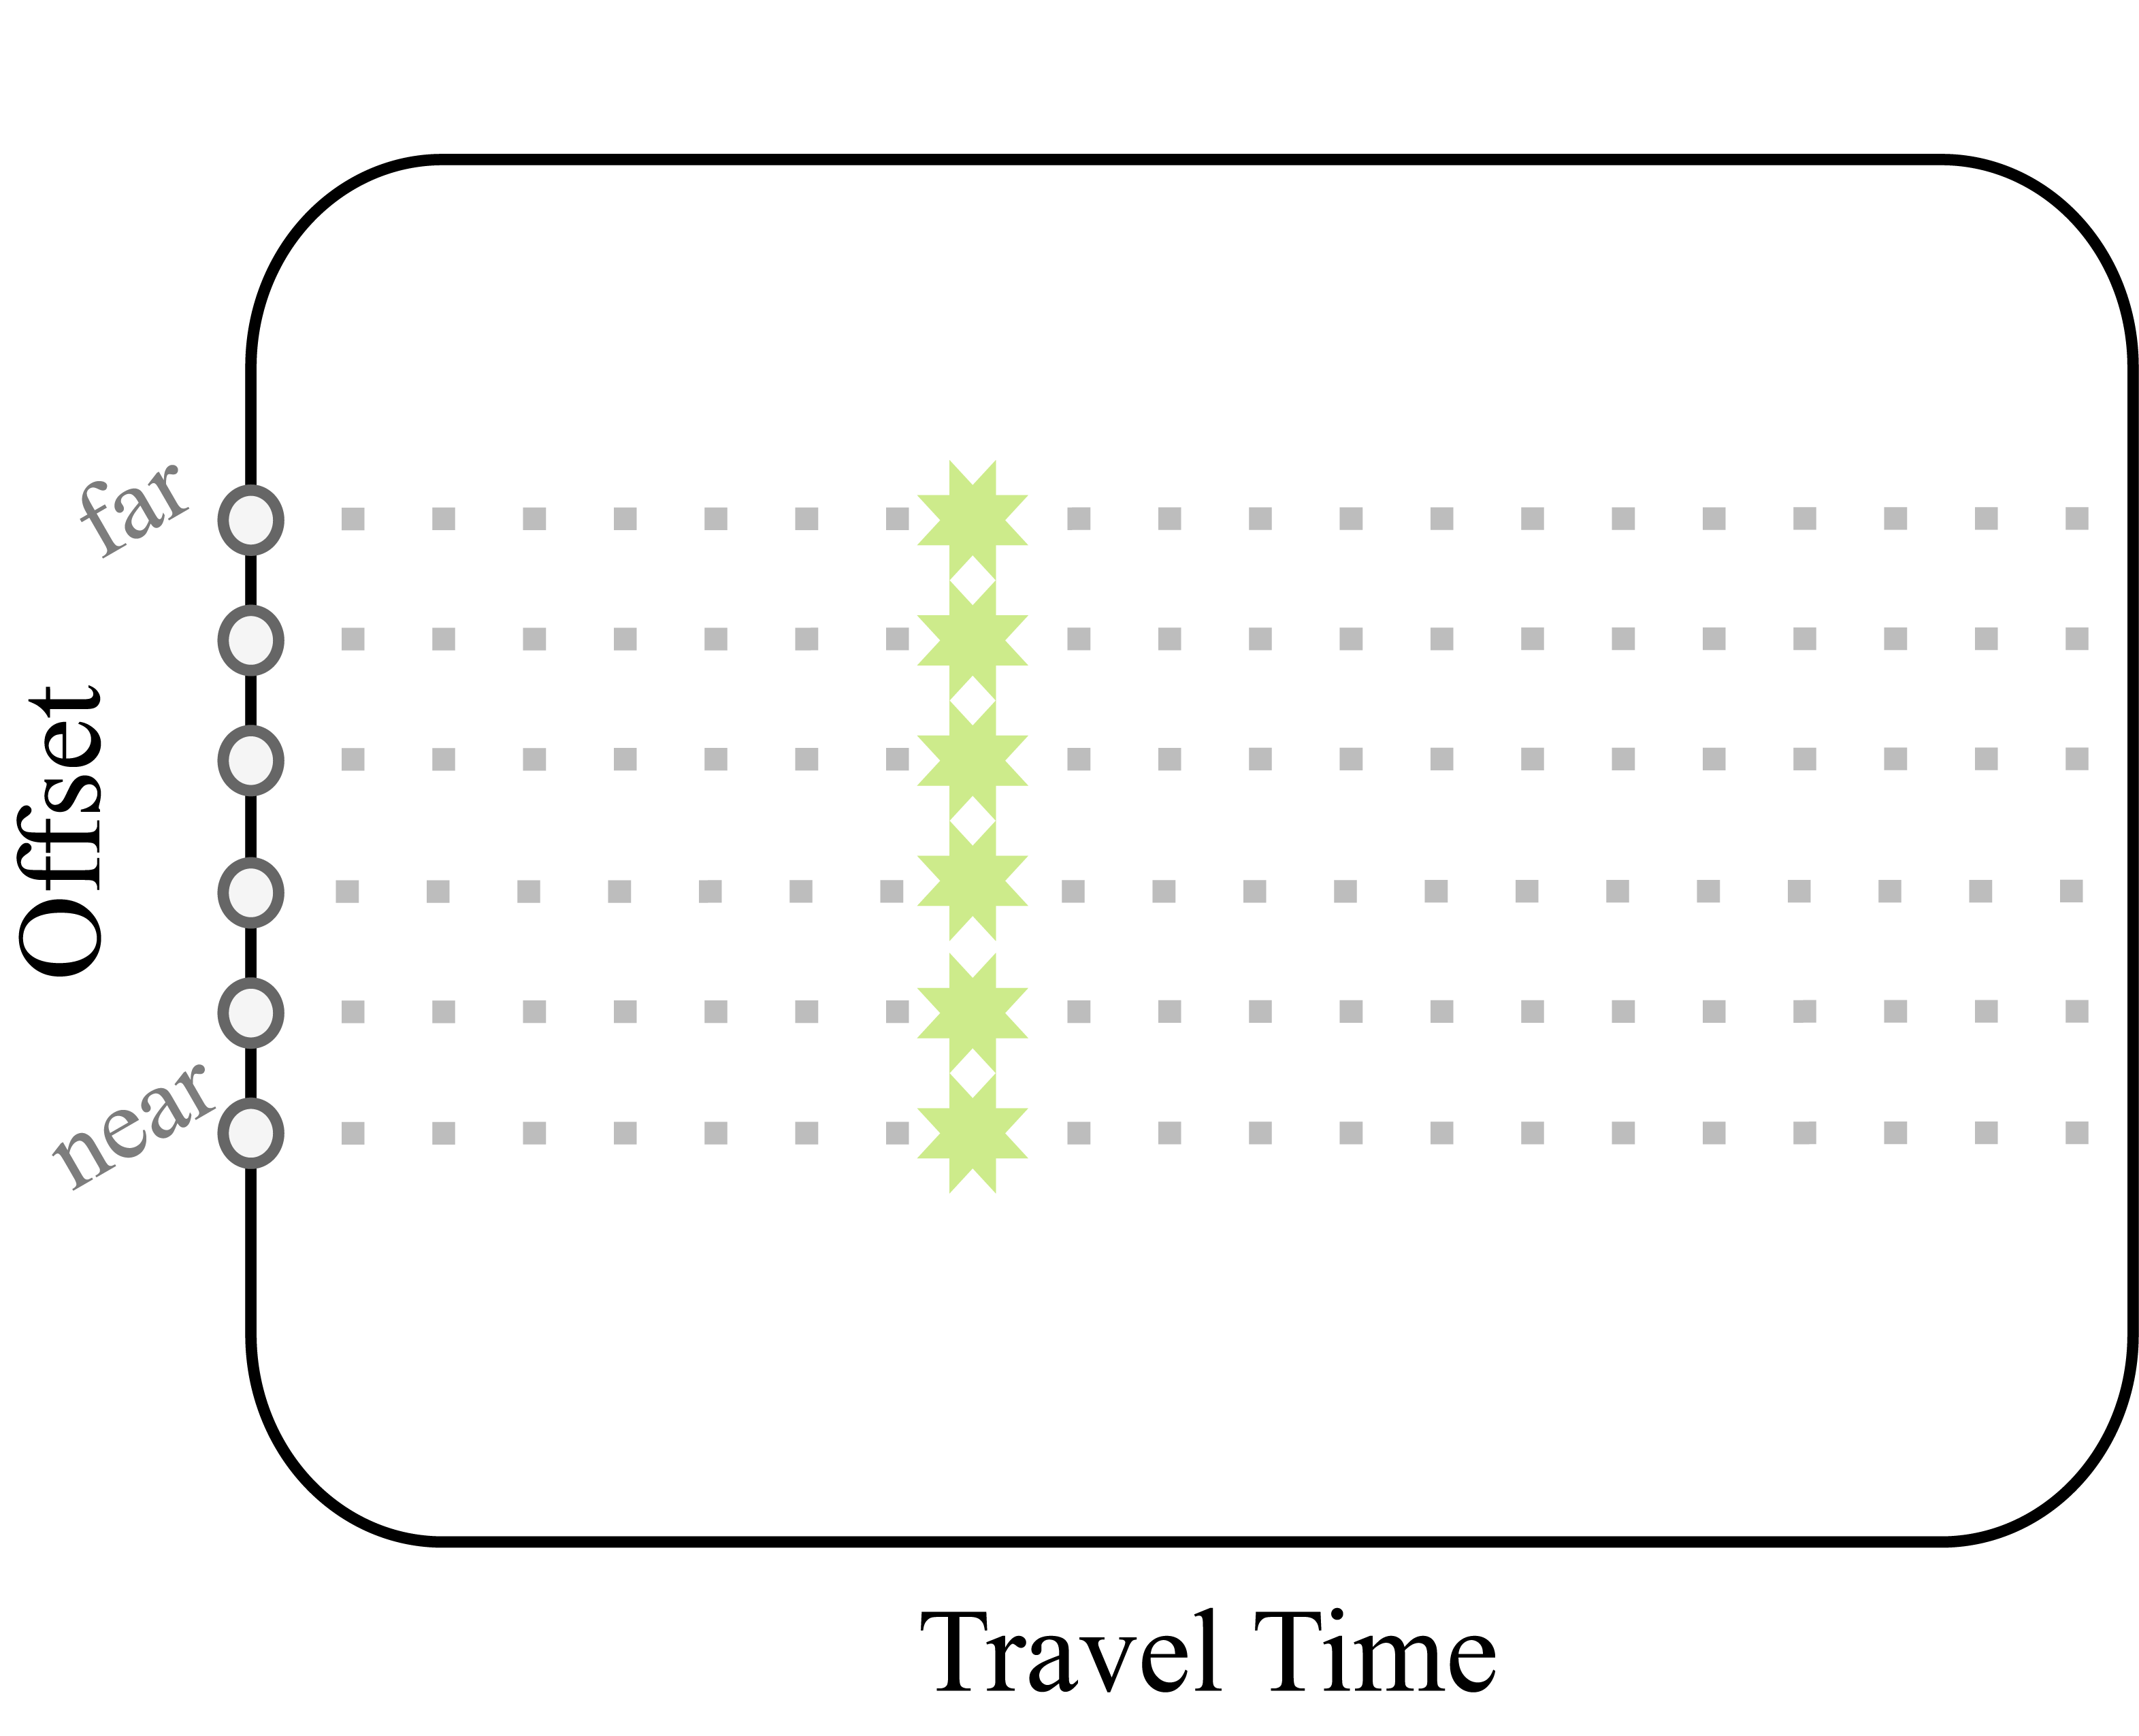
\includegraphics[height=4cm]{05_偏移距与旅行时图像_NMO后.png}
        }
    \end{figure}
\end{frame}

\begin{frame}{速度的选取}
    \begin{figure}[ht]
        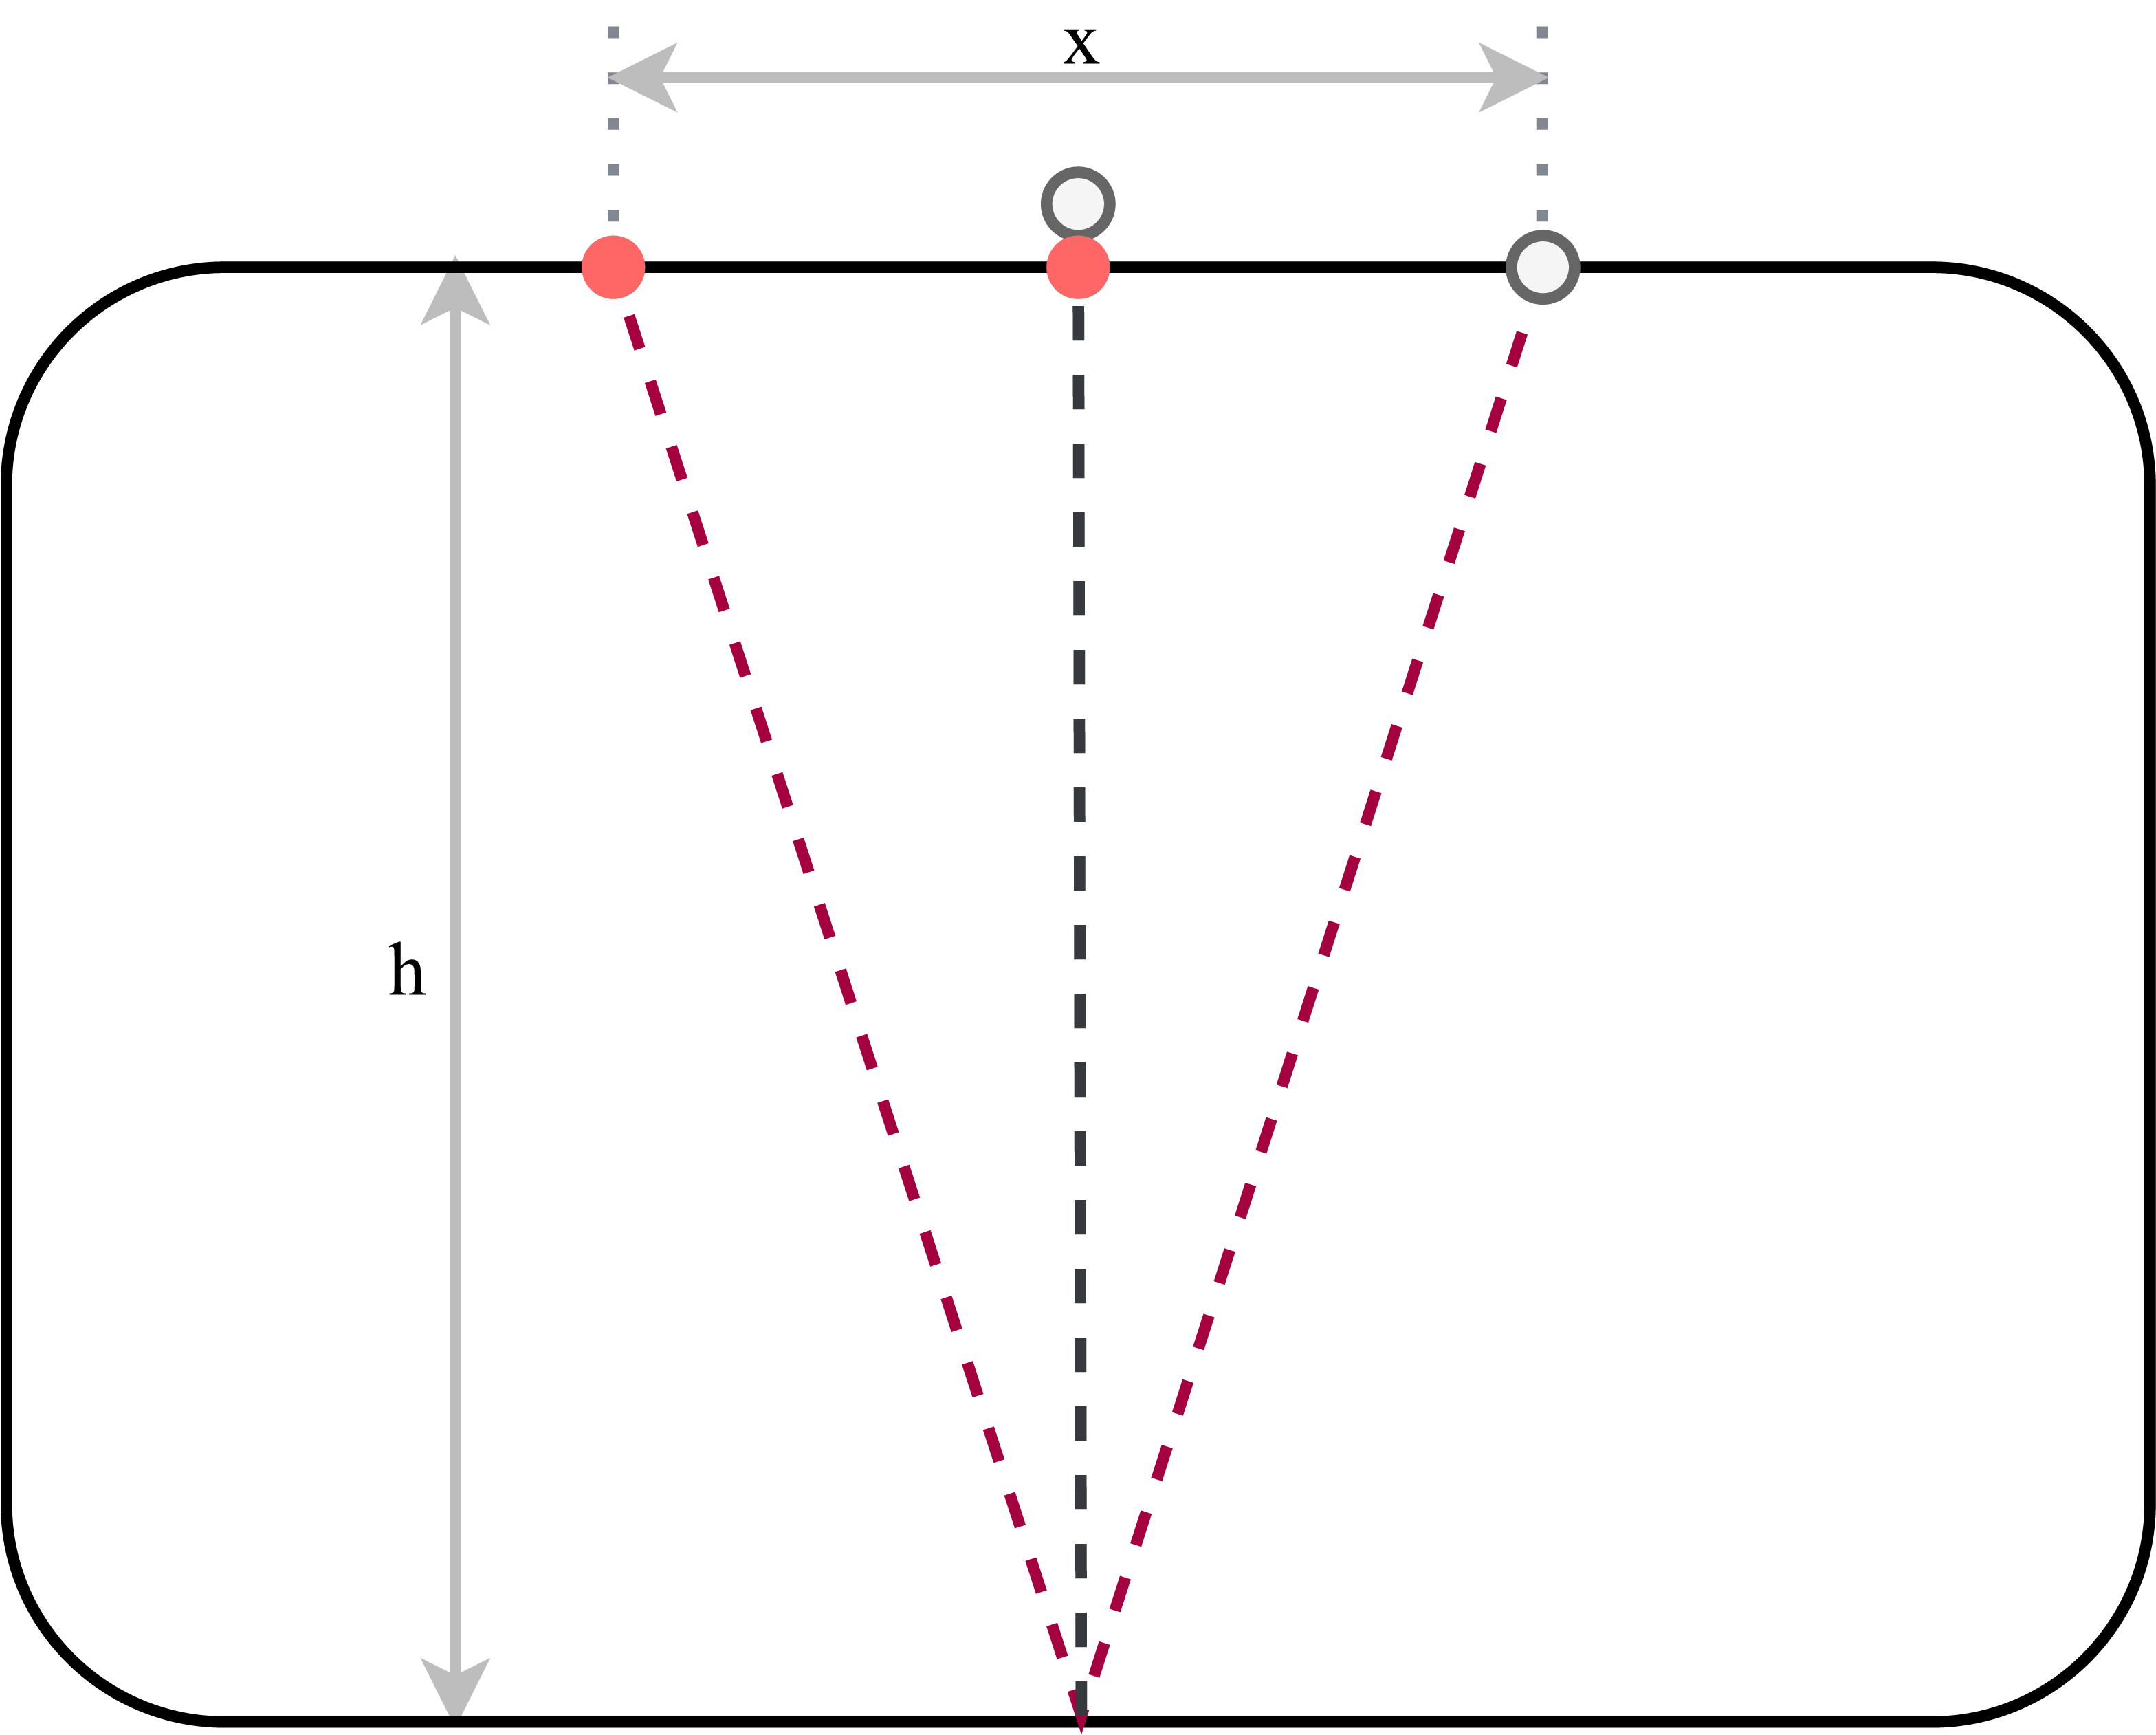
\includegraphics[height=3.5cm]{06_旅行时计算公式.png}
    \end{figure}
    校正后的旅行时$t_0$, 原旅行时$t$, 偏移距$x$, 波速$v$间的关系满足: 
    \[ t_0^2=t^2-\frac{x^2}{v^2} \]
\end{frame}

\begin{frame}{速度的选取}
    \citeauthor{Toldi1989}验证了速度点对应速度谱上的能量峰, 因此对速度点的选择可以转化为在速度谱上进行聚类, 从而寻找聚类中心的问题. 

    \fullcite{Toldi1989}
\end{frame}

% \section{试验介绍}
\begin{frame}{聚类方法}
    \begin{itemize}
        \item K-means
        \item DBSCAN
        \item 基于EM算法的GMM
        \item 基于DP(Dirichlet Process)变分推断的GMM
    \end{itemize}
\end{frame}

\begin{frame}{K-means}
    拟合曲线+原曲线

    拉直图像
\end{frame}

\begin{frame}{DBSCAN}
    
\end{frame}

\begin{frame}{GMM EM}
    
\end{frame}

\begin{frame}{GMM DP}
    
\end{frame}
% \section{其他工作}
\begin{frame}{文献翻译}
    \fullcite{Zhang2016}
    
    \fullcite{Rodriguez2014}
\end{frame}

\begin{frame}{代码}
    \url{https://github.com/Addasecond86/XJTU-Bachelor-Dissertation-Statistics-WangZehao/tree/main/codes}
\end{frame}
 

    \begin{frame}[plain,standout]
        \LARGE \emph{Thanks. }
    \end{frame}

\end{document}
